%%%%%%%%%%%%%%%%%%%%%%%%%%%%%%%%%%%%%%%%%%%%%%%%%%%%%%%%%%%%%%%
%
% Welcome to Overleaf --- just edit your LaTeX on the left,
% and we'll compile it for you on the right. If you open the
% 'Share' menu, you can invite other users to edit at the same
% time. See www.overleaf.com/learn for more info. Enjoy!
%
%%%%%%%%%%%%%%%%%%%%%%%%%%%%%%%%%%%%%%%%%%%%%%%%%%%%%%%%%%%%%%%

\documentclass[12pt, letterpaper]{article}
\usepackage{graphicx} %LaTeX package to import graphics
\usepackage{fontspec}            % Hỗ trợ Unicode và font hệ thống
\usepackage{amsmath}
\usepackage{amssymb}
\usepackage{polyglossia}         % Thay cho babel, hỗ trợ tốt hơn trong XeLaTeX
\setmainlanguage{vietnamese}     % Đặt ngôn ngữ chính
\setmainfont{Times New Roman}    % Chọn font Unicode có sẵn
\graphicspath{{images/}}
\usepackage{amsmath}


\title{My First \LaTeX{} Project}
\author{Pham Nguyen Khanh Minh\thanks{Ha Noi University of Science and Technology.}}
\date{August 8th, 2025}




\begin{document}
\maketitle

\textbf{1. Introduction}


\underline{First document}. This is a simple example with no
extra parameters or packages included.



My name is \textit{Pham Nguyen Khanh Minh}



I am studying at Ha Noi University of Science and Technology. 

\bigskip 

Some of the \textbf{greatest} discoveries in \underline{science} were made by \textbf{\textit{accident}}

\bigskip 

The universe is immense and it seems to be homogeneous, 
on a large scale, everywhere we look.

% The \includegraphics command is 
% provided (implemented) by the 
% graphicx package
\begin{center}
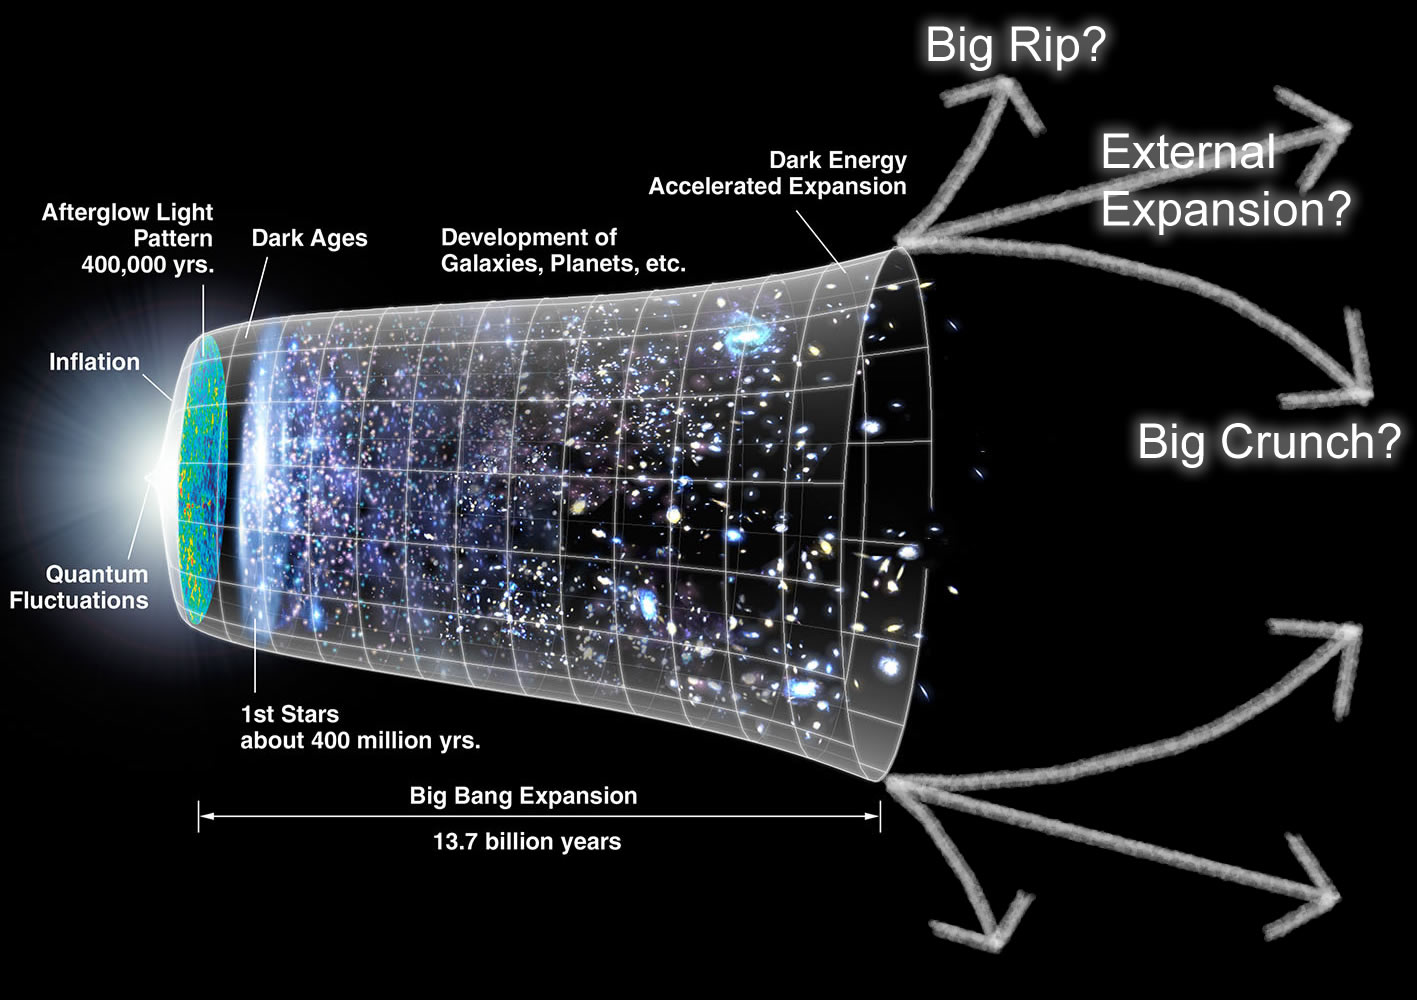
\includegraphics[width=0.5\textwidth]{universe.jpg} 
\end{center}
There's a picture of a galaxy above.

\bigskip

\begin{figure}[ht]
    \centering
    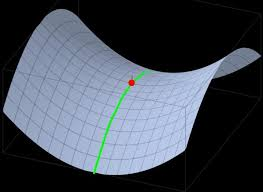
\includegraphics[width=0.5\textwidth]{images/mesh.jpg}
    \caption{Saddle point.}
    \label{fig:mesh1} 
\end{figure}

\newpage 
As you can see in figure \ref{fig:mesh1}, the function grows near the origin.This example is on page \pageref{fig:mesh1}   
    

\begin{itemize}
    \item Một điểm yên ngựa là bất cứ điểm nào mà tất cả gradient của một hàm bằng 0, nhưng đó không phải là một điểm cực tiểu hay giá trị nhỏ nhất
    \item Điểm cực tiểu là vị trí mà ở đó gradient bằng 0 và các trị riêng của ma trận Hessian đều dương
    \item Điểm cực đại là vị trí mà ở đó graident bằng 0 và các trị riêng của ma trận Hessian đều âm.
    \item Điểm yên ngựa là vị trí mà ở đó gradient bằng 0 và các trị riêng của ma trận Hessian mang cả giá trị âm lẫn dương


\end{itemize}

\begin{enumerate}
    \item Hàm mất mát định lượng khoảng cách giữa giá trị thực và giá trị dự đoán của mục tiêu
    \item  Độ mất mát thường là một số không âm và có giá trị càng nhỏ càng tốt. Khi các dự đoán hoàn hảo, chúng sẽ có độ mất mát sẽ bằng 0
    \item Hàm mất mát thông dụng nhất trong các bài toán hồi quy là hàm tổng bình phương các lỗi
\end{enumerate}

\newpage
In Physics, the mass Energy equivalence is stated by the equation $E=mc^2$ discovered in 1905 by Albert Einstien

\bigskip 


Ohm's law $ I = \dfrac{U}{R + r}$ is the relationship between current, voltage, and resistance.



\bigskip
Isaac Newton’s second law of motion is commonly written as 
\[ F=m*a\] where 

\begin{flushleft}
\(F\) is the net force applied to an object,\\
\(m\) is its mass,\\
and \(a\) is the acceleration.
\end{flushleft}

The size of brackets and parentheses can be manually set, or they can be resized dynamically in your document, as shown in the next example:

\[F=G\left(\frac{m_1m_2}{r^2}\right)\]
% This line here is a comment. It will not be typeset in the document.

\newpage
Subscripts in math mode are written as $a_b$  and superscripts are written as $a^b$. These can be combined and nested to write
expressions such as \[T^{i_1 i_2 \dots i_p}_{j_1 j_2 \dots j_q} =
T(x^{i_1},\dots, x^{i_p},e_{j_1},\dots,e_{i_q}) \]

\bigskip 
We write integrals using $\int$ and and fractions using $\frac{a}{b}$. Limits are placed on integrals using superscripts and subscripts

\[\int_{0} ^{1}\frac{dx}{e^{x}} =\frac{e-1}{e} \]
\bigskip
Lower case Greek letters are written as $\lambda$, $\omega$, $\delta$, $\phi$, etc. while upper case Greek letters are written as $\Lambda$,$\Omega$, $\Delta$, $\Phi$

\bigskip
Mathematical operators are prefixed with a backslash as $\sin(\alpha)$, $\cos(\beta)$, $log(x)$, etc.

\newpage
\section{First example}

The well-known Pythagorean theorem \(x^{2}+y^{2}=z^{2}\) was proved to be invalid for other exponents, meaning the next equation has no integer solutions for \(n>2\):

\[x^n+y^n=z^n\]
\section{Second example}
This is a simple math expression \(\sqrt{x^{2}+1}\)  inside text.
And this is also the same: 
\begin{math} 
\sqrt{x^2+1}
\end{math} but by using another command. 

This is a simple math expression without numbering 
\[\sqrt{x^2+1}\] separated from text.


This is also the same:
\begin{displaymath}
\sqrt{x^2+1}
\end{displaymath}
\ldots and this:

\begin{equation*}
\sqrt{x^2+1}    
\end{equation*}


Subscripts and superscripts can be nested and combined in various ways. When nesting subscripts/superscripts, however, remember that each command must refer to a single element; this can be a single letter or number, as in the examples above, or a more complex mathematical expression collected in braces or brackets. For example:

\[(a^n)^{r+s}=a^{nr+ns} \]


Some mathematical operators may require subscripts and superscripts. The most frequent cases are those of the integral (check the introduction) and the summation operators, whose bounds are typeset precisely with subscripts and superscripts.


\[\sum_{i=1}^{\infty} \frac{1}{n^s} =\prod_{p} \frac{1}{1-p^{-s}} \]

Here are some examples of simple usage of subscripts and superscripts:

\[ \int\limits_0^1 x^2 + y^2 \ dx \]


Using superscript and subscripts in the same expression

\[ a_1^2 + a_2^2 = a_3^2 \]

\vspace{1cm}

Squared root usage

\[ \sqrt[4]{4ac} = \sqrt{4ac}\sqrt{4ac} \]

Pipes; vertical bars	|x+y|

Double pipes \|x+y\|




The possibilities with math in \LaTex{} are endless so be sure to visit our help pages for advice and examples on specific topics

\bigskip

Notice that to insert the parentheses or brackets, the left and right commands are used. Even if you are using only one bracket, both commands are mandatory. left and right can dynamically adjust the size, as shown by the next example:

\[
\left[  \frac{N} { \left( \frac{L}{P}  \right) -\left( m+n \right ) }\right]
\]

\begin{align*}
y  = 1 + & \left(  \frac{1}{x} + \frac{1}{x^2} + \right. \frac{1}{x^3}  + \ldots  \\
  & \left. \quad  + \frac{1}{x^{n-1}} + \frac{1}{x^n} \right)
\end{align*}


%-------------------------------------------------------%
\newpage
This article explains how to typeset fractions and binomial coefficients, starting with the following example which uses the


The binomial coefficient, \(\binom{n}{k}\)  is defined by the expression:

\[\binom{n}{k} = \frac{n!}{k!  \left(n-k \right)!}\]




Fractions typeset within a paragraph typically look like this:
\(\frac{3x}{2}\)

You can force \LaTeX{} to use the larger display style,
such as \(\displaystyle \frac{3x}{2} \), which also has an effect on line spacing. The size of maths in a paragraph can also be reduced: \(\scriptstyle \frac{3x}{2}\) or \(\scriptscriptstyle \frac{3x}{2}\). 


For the verb scriptscriptstyle example note the reduction in spacing: characters are moved closer to the \textit{vinculum} (the line separating numerator and denominator).


Equally, you can change the style of mathematics normally typeset in display style:


\[f(x)=\frac{P(x)}{Q(x)}\quad \textrm{and}\quad \textstyle
f(x)=\frac{P(x)}{Q(x)}\quad \textrm{and}\quad \scriptstyle
f(x)=\frac{P(x)}{Q(x)}
\]



Fractions can be nested but, in this example, note how the default math styles, as used in the denominator, don't produce ideal results...


\[\frac{1+\frac{a}{b}} {1+\frac{1}{1+\frac{1}{a}}}\]


\noindent ...so we use \verb|\displaystyle| to improve typesetting:

\[\frac{1+\frac{a}{b}} {\displaystyle 1+\frac{1}{1+\frac{1}{a}}}\]

Here is an example which uses the \texttt{amsmath} \verb|\cfrac| command:


\[a_0+\cfrac{1}{a_1+\cfrac{1}{a_2+\cfrac{1}{a_3 +\cdots}}}\]

Here is another example, derived from the \texttt{amsmath} documentation, which demonstrates left
and right placement of the numerator using \verb|\cfrac[l]| and \verb|\cfrac[r]| respectively:

\newpage 
The amsmath package provides a handful of options for displaying equations. You can choose the layout that better suits your document, even if the equations are really long, or if you have to include several equations in the same line.
Let's start with a basic example:



\begin{equation} \label{eq1}
\begin{split}
A & = \frac{\pi r^2}{2}  \\
 & = \frac{1}{2} \pi r^2 
\end{split}
\end{equation}


To display a single equation, as mentioned in the introduction, you have to use the equation* or equation environment, depending on whether you want the equation to be numbered or not. Additionally, you might add a label for future reference within the document.

\begin{equation} \label{eu_eqn}
e^{\pi i}+1=0    
\end{equation} 

The beautiful equation \ref{eu_eqn} is known as the Euler equation.

\bigskip
\textbf{Display long equation}

For equations longer than a line use the multline environment. Insert a double backslash to set a point for the equation to be broken. The first part will be aligned to the left and the second part will be displayed in the next line and aligned to the right.

Again, the use of an asterisk * in the environment name determines whether the equation is numbered or not.
The beautiful equation \ref{eu_eqn} is known as the Euler equation.
\begin{multline*}
p(x) = 3x^6 + 14x^5y + 590x^4y^2 + 19x^3y^3\\ 
- 12x^2y^4 - 12xy^5 + 2y^6 - a^3b^3
\end{multline*}

\textbf{Aligning several equations}

If there are several equations that you need to align vertically, the align environment will do it:

\begin{align}
    2x-5y&=8\\ 
    3x-12y&=9
\end{align}

Usually the binary operators (>, < and =) are the ones aligned for a nice-looking document.

As mentioned before, the ampersand character  determines where the equations align. Let's check a more complex example:

\begin{align*}
    x&=y          & w&=z                  & a&=b+c\\ 
    2x&=-v        & 3w&=\frac{1}{2}z      & a&=b\\
    -4 + 5x&=2+y  & w+2&=-1+w             & ab&=cb
\end{align*}


Here we arrange the equations in three columns. LaTeX assumes that each equation consists of two parts separated by an  and that each equation is separated from the one before by an .


Again, use * to toggle the equation numbering. When numbering is allowed, you can label each row individually.



\textbf{Grouping and centering equations}

If you just need to display a set of consecutive equations, centered and with no alignment whatsoever, use the gather environment. The asterisk trick to set/unset the numbering of equations also works here.

\begin{gather*} 
2x - 5y =  8 \\ 
3x^2 + 9y =  3a + c
\end{gather*}


Examples of mathematical operators:

\[
      \sin(a+b) =\sin(a)\cos(b) +\sin(b)\cos(a)
\]

Some operators can take parameters that are handled in a special way, for instance, limits.

Testing notation for limits:
\[
    \lim_{h \to 0 } \frac{f(x+h)-f(x)}{h}
.\]

This operator changes when used alongside 
text \(\lim_{h \to 0} \left( x-h \right)\)


\newpage
\textbf{Integrals}

Note, that integral expression may seems a little different in inline and display math mode.
Intergral \(\int_{a}^{b} x^2\, dx \) inside text

To obtain double/triple/multiple integrals and cyclic integrals you must use amsmath and esint (for cyclic integrals) packages.



\begin{gather}
    \iint_V \mu(u,v) \,du,\,dv
\\
    \iint_V \mu(u,v,w) \,du\,dv \,dw
\\
    \iiint_V \mu(u,v,t,w) \,du \, dv\,dt\,dw
\\
    \idotsint_V \mu(u_1,\dots,u_k) \,du_1 \dots du_k
\end{gather}

\[
    \oint_V f(s) \,ds
\]


\textbf{Sum and Product}

Sum  \(\sum_{n=1}^{\infty} 2^{-n}=1\) inside text

\medskip
In similar way you can obtain expression with product of a sequence of factors using the 

Product \(\prod_{i=a}^{b} f(i)\) inside text

\medskip

Limit $\lim_{x\to\infty} f(x)$ inside text


Some mathematical elements need to be typeset using fonts containing characters/symbols of a certain style; for example, it is customary to represent real numbers with a blackboard bold font (such as ), or topological spaces with calligraphic font 

This article shows how to use different font styles when typesetting mathematics, starting with the following example:

Let \(\mathcal{T}\) be a topological space, a basic is defined 
as 
\[
    \mathcal{B} = \{B_{\alpha} \in \mathcal{T}\, |\,  U=\bigcup B_{\alpha} \forall  U \in \mathcal{T} \}
\]

\newpage

\textbf{Capital letters-only font typefaces}

There are some font typefaces which support only a limited number of characters; these fonts usually denote some special sets. For instance, to display the R in blackboard bold typeface you can use mathbb{R} to produce 

. The following example shows calligraphic, fraktur and blackboard bold typefaces:




\begin{align}
RQSZ \\
\mathcal{RQSZ} \\
\mathfrak{RQSZ} \\
\mathrm{RQSZ} \\
\mathbb{RQSZ}\\
\end{align}

\textbf{Other math front }

\begin{align*}
3x^2 \in R \subset Q \\
\mathnormal{3x^2 \in R \subset Q} \\
\mathrm{3x^2 \in R \subset Q} \\
\mathit{3x^2 \in R \subset Q} \\
\mathbf{3x^2 \in R \subset Q} \\
\mathsf{3x^2 \in R \subset Q} \\
\mathtt{3x^2 \in R \subset Q}
\end{align*}


\end{document}